\section{Customer instructions}
\subsection{Signing out}
An authenticated user can sign out from the platform. To perform this action the user needs to click the sign-out button that is present in the header. When the button is pressed user is logged out form platform.
\begin{figure}[!ht]
    \caption{Header}
    \vspace{10px}
    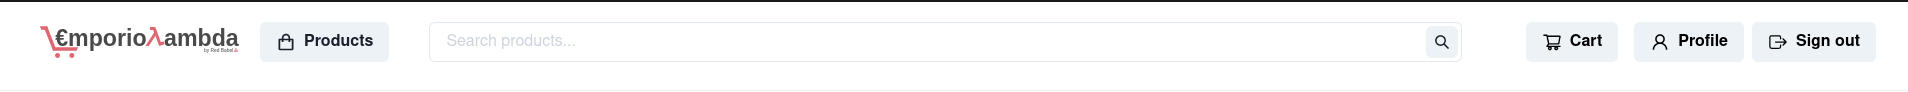
\includegraphics[scale=0.25]{../../../../Images/userManual/signOut.jpg}
    \centering
\end{figure}
\subsection{Viewing and editing user data}
An authenticated user can view and modify his data.
\subsubsection{Viewing user data}
To perform this action the authenticated user has to click the profile button.
\begin{figure}[!ht]
    \caption{Button detail}
    \vspace{10px}
    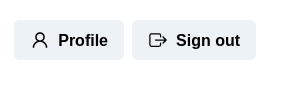
\includegraphics[scale=0.5]{../../../../Images/userManual/profile-signoutButton.png}
    \centering
\end{figure}
When the button is pressed the user see the dashboard page, were all his data is shown.
\begin{figure}[!ht]
    \caption{User data}
    \vspace{10px}
    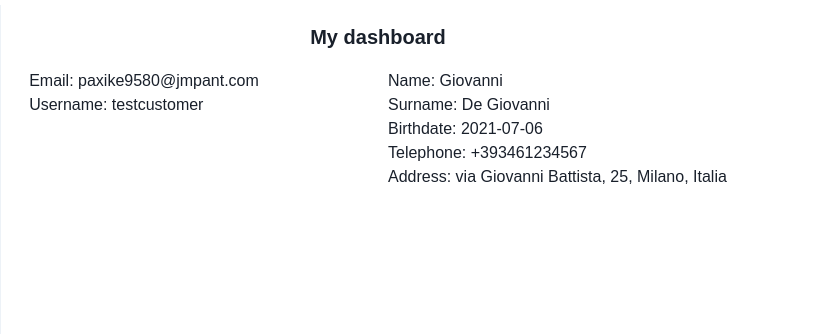
\includegraphics[scale=0.5]{../../../../Images/userManual/profileDshboard.png}
    \centering
\end{figure}
\newpage
\subsubsection{Modify user data}
When user is in the profile page he can press the \textit{Edit profile} button present in the profile navbar\textsubscript{\textbf{G}}.
\begin{figure}[!ht]
    \caption{Profile page navbar}
    \vspace{10px}
    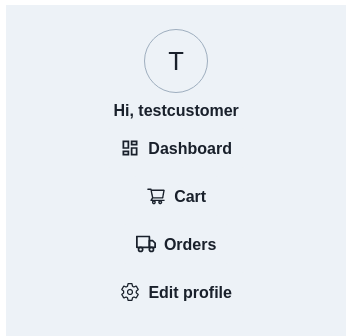
\includegraphics[scale=0.5]{../../../../Images/userManual/dashboardNavBar.png}
    \centering
\end{figure}
When the button is pressed the user see the page for modify his data. He can change the data that he wants to modify using the proper form.
\begin{figure}[!ht]
    \caption{Profile page navbar}
    \vspace{10px}
    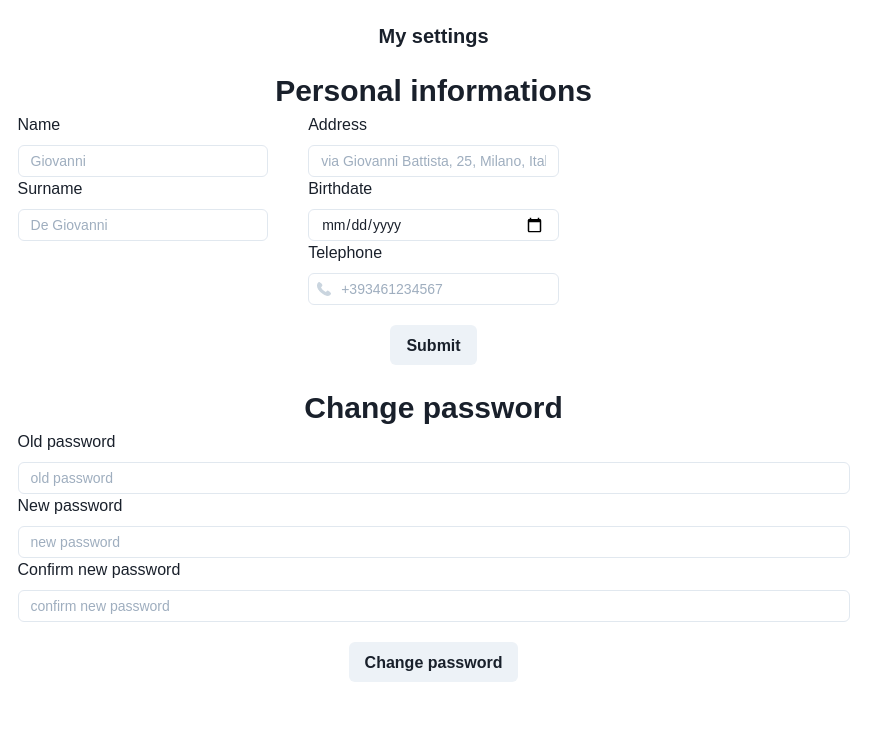
\includegraphics[scale=0.3]{../../../../Images/userManual/profileModfication.png}
    \centering
\end{figure}
\\
When he clicks the submit button a pop-up appears to indicate the result of the action. With the popup the user can return to the profile dashboard.
\newpage
\subsection{Check out}
An authenticated user can perform the checkout. To perform this action the user must be logged, and he has to be in the cart page.
\begin{figure}[!ht]
    \caption{Cart page}
    \vspace{10px}
    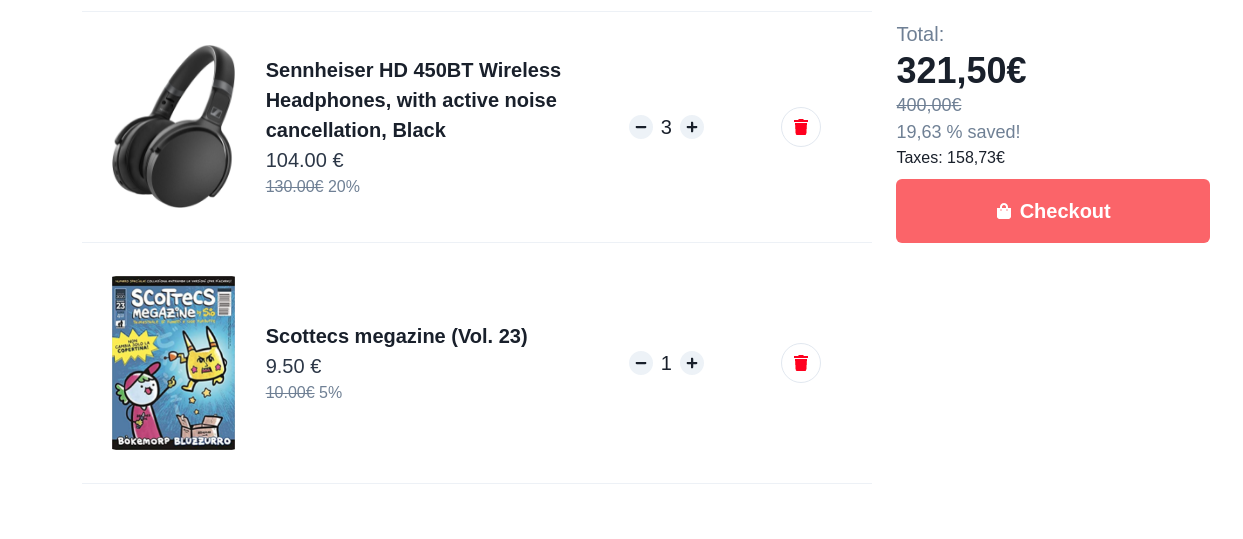
\includegraphics[scale=0.35]{../../../../Images/userManual/cart.png}
    \centering
\end{figure}
\\
He can press the checkout button that redirect him to the stripe checkout.
\begin{figure}[!ht]
    \caption{Checkout}
    \vspace{10px}
    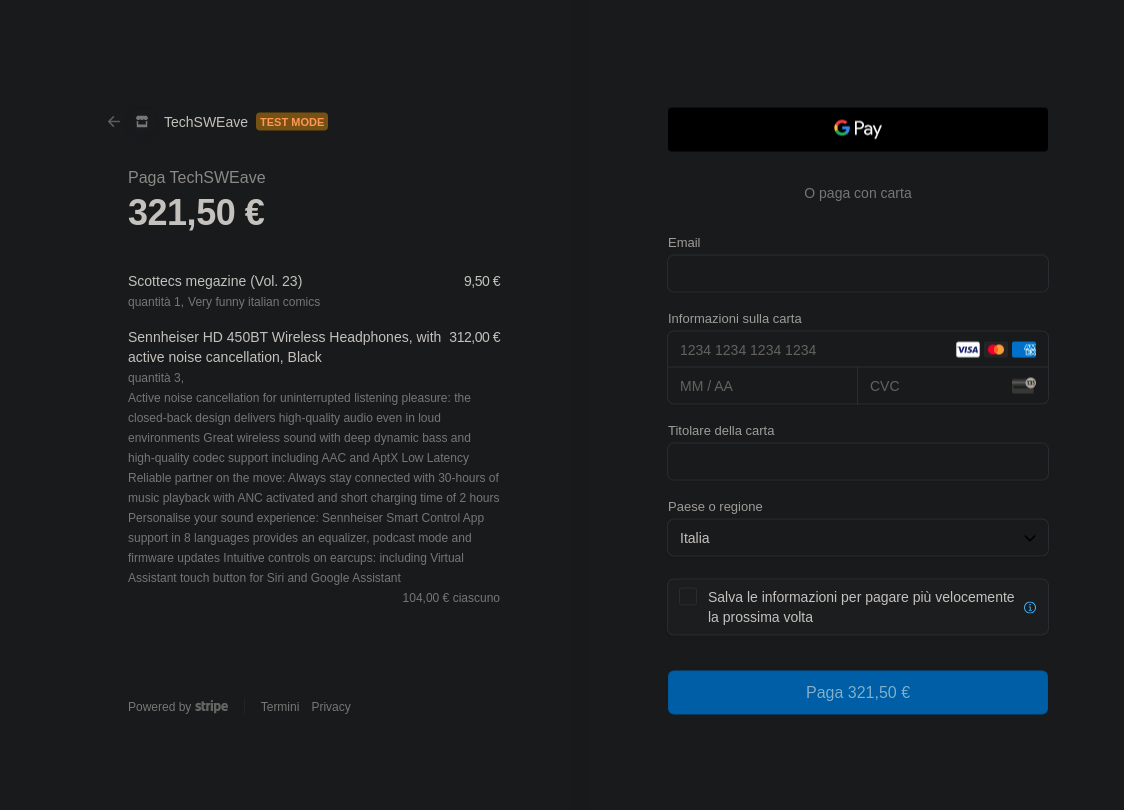
\includegraphics[scale=0.3]{../../../../Images/userManual/checkout.png}
    \centering
\end{figure}
\\
The user now has to insert:
\begin{itemize}
    \item e-mail;
    \item card number;
    \item expiration date:
    \item CVC;
    \item name.
\end{itemize}
The user can also use other payment method like \textit{Gpay} and \textit{Apple Pay}.
When the user entered all the required information he can click the checkout payment button to pay the order. After this he is redirected to the success page and here he can go to his order page list, or if the checkout fail to the cart page.
\begin{figure}[!ht]
    \caption{Checkout success}
    \vspace{10px}
    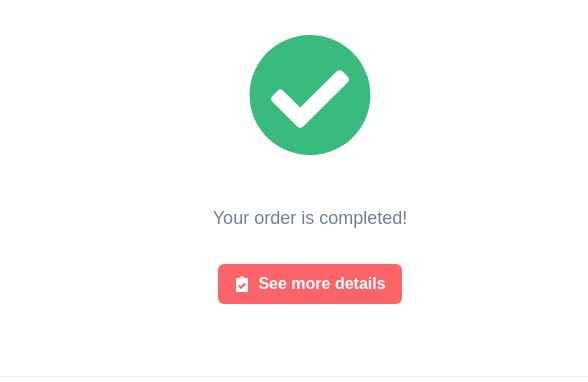
\includegraphics[scale=0.5]{../../../../Images/userManual/checkoutSuccess.png}
    \centering
\end{figure}
\subsection{Order list visualization}
An authenticated user can view all his previous order. To perform this action the user has to be in the profile page, and he has to click the \textit{order} button.
\begin{figure}[!ht]
    \caption{Profile page navbar}
    \vspace{10px}
    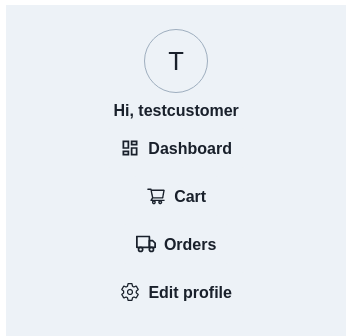
\includegraphics[scale=0.5]{../../../../Images/userManual/dashboardNavBar.png}
    \centering
\end{figure}
\newpage
When the button is pressed the order list is shown. There is two different view for order list depending on the device in use.
\begin{itemize}
    \item Desktop visualization:
          the user see all his order with product information like:
          \begin{figure}[!ht]
              \caption{Desktop order}
              \vspace{10px}
              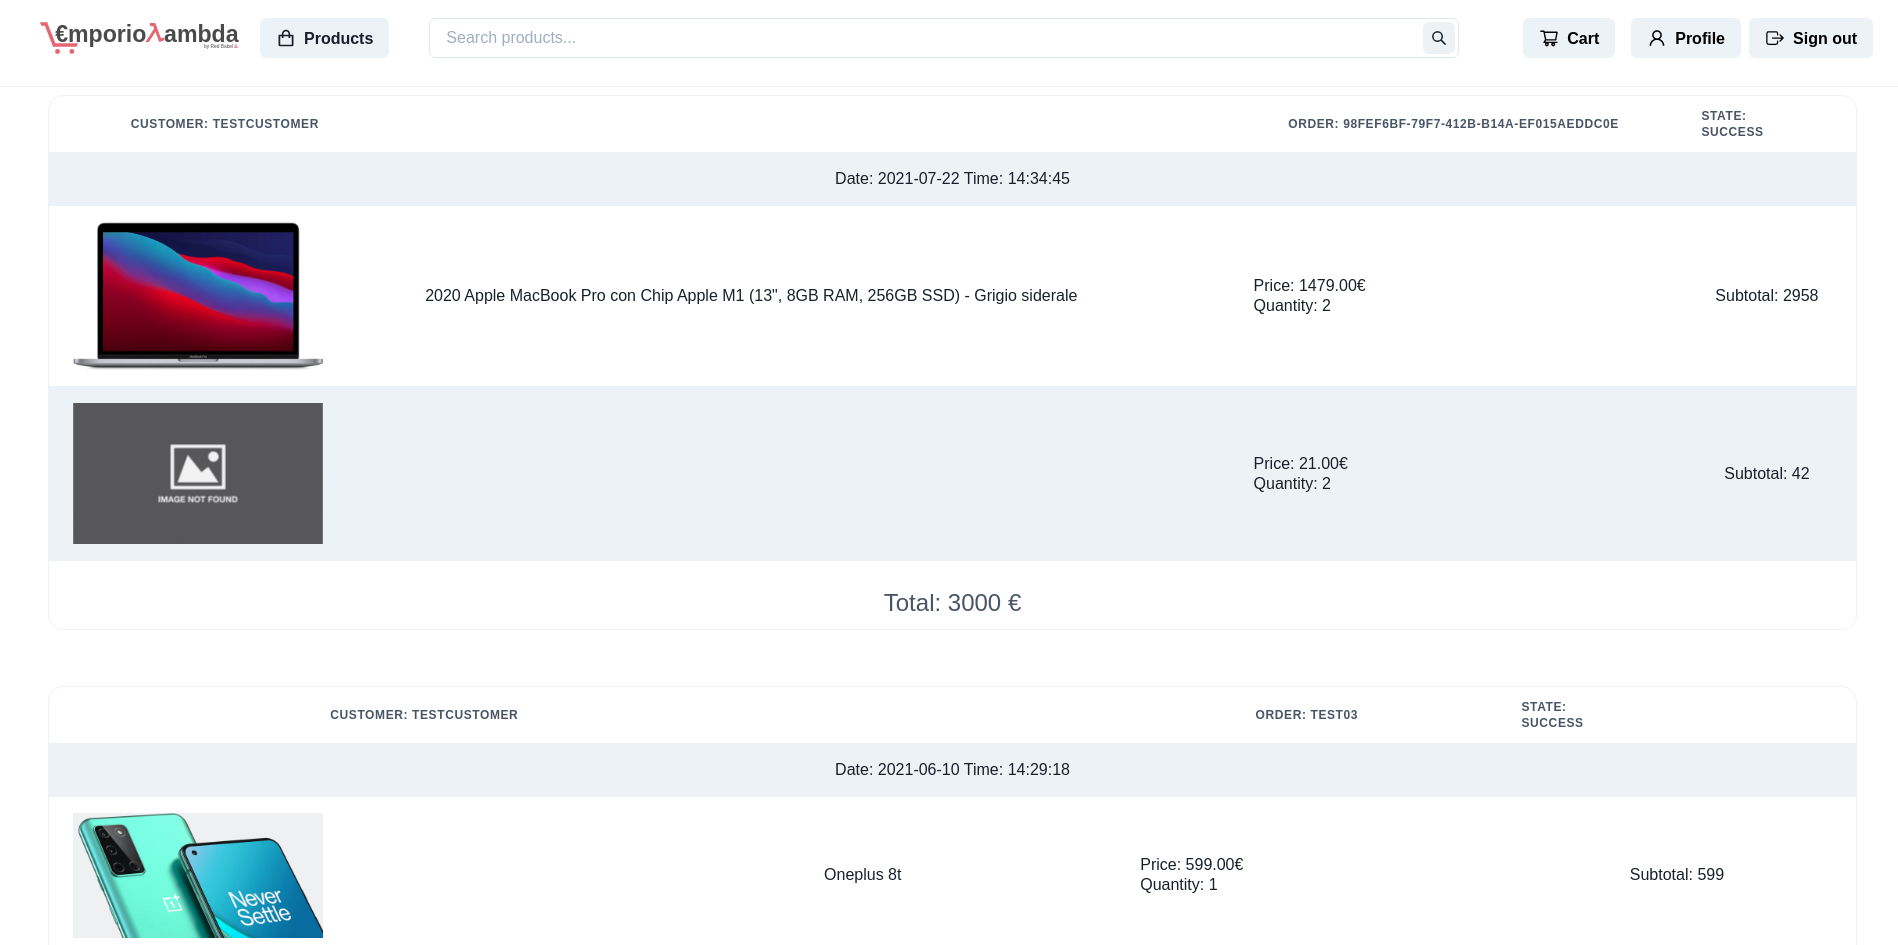
\includegraphics[scale=0.2]{../../../../Images/userManual/orderDesktop.png}
              \centering
          \end{figure}
          \\
          \begin{itemize}
              \item username;
              \item order ID;
              \item order date;
              \item title;
              \item image;
              \item price;
              \item quantity;
              \item description;
              \item order state;
              \item total of the single product;
              \item total of the order;
          \end{itemize}
          \newpage
    \item Mobile visualization
          \begin{figure}[!ht]
              \caption{Mobile order}
              \vspace{10px}
              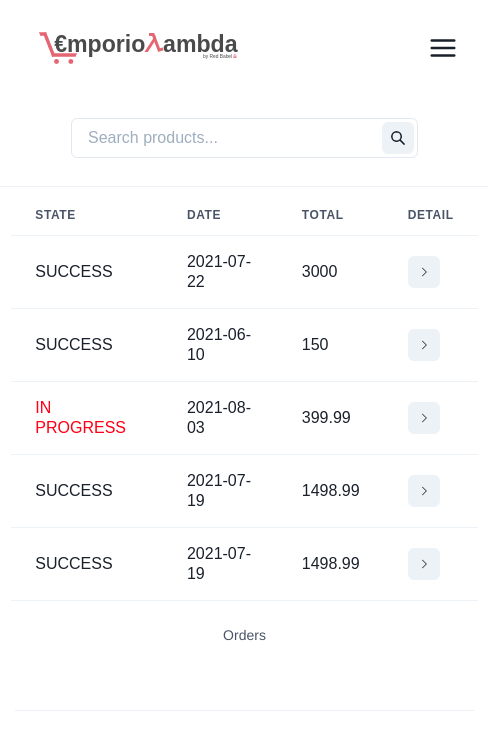
\includegraphics[scale=0.3]{../../../../Images/userManual/orderMobile.png}
              \centering
          \end{figure}
          the user see an order list with:
          \begin{itemize}
              \item order state;
              \item order date;
              \item total;
              \item detail button.
          \end{itemize}
          When the user from mobile clicks the detail button he is redirected to the order detail where he can see all the order information like desktop visualization.
          \begin{figure}[!ht]
              \caption{Mobile order detail}
              \vspace{10px}
              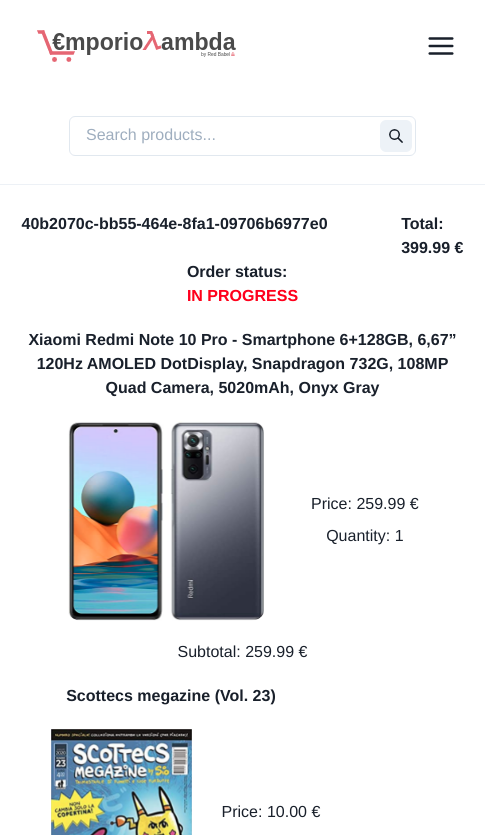
\includegraphics[scale=0.2]{../../../../Images/userManual/oderMobileDetail.png}
              \centering
          \end{figure}

\end{itemize}
